\chapter{Execução da Pesquisa e Resultados da Fase 1}

\section{Execução da Pesquisa}

\subsection{Kanban}

Na primeira semana, foi elaborado um quadro kanban para podermos gerenciar e termos melhor controle sobre as atividades a serem feitas.

O quadro foi montado possuindo as seguintes colunas: Backlog, A fazer, em andamento, revisão por pares, revisão, correção e concluído.

Primeiramente foi mapeado o fluxo, elencando as atividades a serem feitas e entregues. Estas atividades foram colocadas na coluna de "Backlog". Logo após, os requisitos foram separados por conteúdo e prioridade, sendo as atividades de maior prioridade as que estavam no topo da coluna de backlog.

Ao terminar de montar o backlog, as atividades que começaram a serem feitas foram para a coluna de "A fazer", com o prazo de uma semana para a conclusão dos artefatos presentes nesta coluna.

\subsection{Validação com o orientador}

Após a elaboração inicial do questionário, foi realizado uma validação por parte do docente em que foram identificadas oportunidades de melhorias e correção de incongruências ou questões que estivessem desconexas com o propósito do formulário.

\subsection{Grupo Focal}

Como referenciado no capítulo de Metodologias, a primeira etapa do grupo focal deve ser o planejamento e a definição do objetivo do grupo focal. O objetivo da atividade foi discutir como melhorar os feedbacks nas avaliações individuais na plataforma do Moodle usando Inteligência Artificial, em que o foco foi em decidir como fornecer feedbacks mais úteis e construtivos aos alunos, com o objetivo de aprimorar a aprendizagem e o envolvimento na plataforma.

O moderador foi o responsável por montar o roteiro que guiou todo o grupo focal, assim como pelo recrutamento dos participantes.

O local selecionado para a realização do grupo focal foi a sala S6, localizada na Universidade de Brasília no campus do Gama, uma sala grande, em que foi possivel organizar as cadeiras em formato semi-circular, facilitando, assim, o contato visual entre todos os presentes.

As personas que participaram do grupo focal foram alunos da Universidade de Brasília do campus do Gama que cursam ou cursaram as disciplinas de Métodos de Desenvolvimento de Software ou Requisitos de Software com o professor George Marsicano Correa.

Para a obtenção de voluntários, foi passada uma lista em que os alunos que desejassem participar deveriam colocar seu nome e número de celular. Após a coleta das informações dos voluntários, foi criado um grupo na plataforma do WhatsApp para verificar a disponibilidade dos participantes, e assim, encontrar um dia e hora em que fosse possível a participação da maior quantidade de voluntários, com isso, conseguimos a confirmação de dez estudantes que se comprometeram a participar do grupo focal no dia e no horário combinados.

No dia da execução do grupo focal, nenhum dos dez estudantes, que haviam se comprometido, compareceram, mesmo mediante diversas mensagens de lembrança e pedidos para que avisassem caso não pudessem estar presentes. Três dos dez alunos avisaram no dia em questão que não poderiam ir, e os demais nem sequer avisaram, mesmo após o horário.

Mediante este problema, foram convidados alguns alunos para participarem do grupo focal, e dentre estes, quatro aceitaram o convite e participaram, sendo todos estes ex-estudantes das disciplinas de MDS ou RS com o professor George Marsicano.

No início, foi distribuído, para cada participante, um termo de consentimento para gravação da reunião em questão, e após todos assinarem, a gravação foi iniciada, tendo, no final, uma duração de quarenta minutos. O grupo focal foi guiado mediante um roteiro préviamente elaborado contendo as seguintes etapas:

1. Introdução: Nesta parte ocorreram as saudações e boas-vindas aos participantes, apresentação do objetivo da entrevista e contexto do tema, e a realização de um quebra-gelo para que os estudantes se sentissem mais confortáveis.

2. Conhecendo os Participantes: Breve apresentação de cada participante.

3. Experiências passadas: Nesta etapa os dicentes foram questionados sobre experiências passadas em avaliações individuais e o feedback recebido. Além disso, foi explorado como o feedback recebido influenciou o desenvolvimento pessoal e profissional. 

4. Percepções sobre o Feedback Atual: Foi perguntado sobre a eficácia do feedback fornecido em avaliações individuais. 

5. Identificação de Desafios: Questionamento sobre os principais desafios enfrentados ao receber feedback em avaliações individuais. Também foi explorado se os desafios estão relacionados à clareza, relevância, ou outro aspecto do feedback. 

6. Sugestões para Aprimoramento: Nesta etapa foi solicitado sugestões dos participantes sobre como o feedback poderia ser aprimorado para ser mais útil e eficaz. Também foi incentivado a discussão sobre métodos inovadores ou abordagens que possam melhorar o processo de feedback. 

7. Compreensão das Preferências: Perguntar sobre as preferências individuais em relação à entrega do feedback.

8. Encerramento: Agradecimento a participação dos entrevistados e também foi oferecido oportunidade para os participantes adicionarem quaisquer comentários finais. 

Após a conclusão do grupo focal, foi percebido que a quantidade de participantes e a amostra da população presente não foram as ideias, O esperado era a participação de no mínimo seis participantes, e foram obtidos apenas quatro, além disso, os participantes deveriam ser estudantes das disciplinas de MDS e RS no semestre vigente, porém, os discentes que participaram eram todos alunos que já haviam concluido estas disciplinas.

Tendo em vista os problemas citados, foi realizada uma nova tentativa para a realização de um novo grupo focal com os estudantes que não puderam comparecer, porém, apenas quatro pessoas foram voluntárias, não sendo possível atingir o mínimo de participantes desejados na grupo focal.

Após o grupo focal, foram feitas correções e adições no formulário, o qual passou novamente por uma validação com o docente para confirmação das alterações.

Com as validações concluídas, o formulário foi liberado para que a população amostral escolhida respondesse as perguntas. Os participantes foram todos alunos das disciplinas de Métodos de Desenvolvimento de Software, de código FGA0138, e Requisitos de Software, de código FGA0172, ambas ministradas pelo professor George Marsicano Corrêa. No total foram obtidas setenta de duas respostas.

\subsection{Seleção de artigos}

Para a elaboração do formulário foram aplicadas diversas técnicas com embasamento teórico e acadêmico. Para encontrar estes estudos, foram seguidas as seguintes práticas:

1. Identificação de Bases de Dados e Repositórios: Seleção de bases de dados acadê-
micas reconhecidas, como Scopus, Web of Science, Google Scholar, entre outras.

2. Definição de Palavras-chave e Categorias: Palavras como "feedback", "aprendiza-
gem", "feedback formativo", "feedback somativo", "feedback descritivo", entre outras, foram
utilizadas para filtrar pesquisas relevantes.

3. Seleção Preliminar de Artigos: Os títulos, resumos dos artigos e quantidade de
citações foram analisadas para determinar sua relevância para o estudo.

4. Leitura e Análise Detalhada: Artigos selecionados foram lidos integralmente para
extração de insights e práticas pertinentes.

5. Síntese e Categorização: As informações coletadas foram sintetizadas e categori-
zadas para facilitar sua aplicação prática na definição de feedbacks no Microsoft Forms.
Baseando-se nas descobertas da pesquisa em artigos, os feedbacks no Microsoft
Forms foram estruturados de forma a maximizar a eficácia e o impacto positivo no apren-
dizado dos alunos. A decisão sobre qual tipo de feedback priorizar foi tomada com base
na literatura e adaptada ao contexto específico do TCC.

6. Snowballing:  A técnica de snowballing foi utilizada no trabalho para encontrar novos estudos relevantes a partir da análise de referências em trabalhos já existentes.

Aplicando as etapas de iteração do backward snowballing, citadas no capítulo de Metodologias, os seguintes artigos utilizados como referência neste trabalho foram encontrados:

1. "Survey research methodology in management information systems: an assessment" \cite{pinsonneault1993survey}.

2. "A avaliação da confiabilidade de questionários: uma análise utilizando o coeficiente alfa de cronbach" \cite{freitas2005avaliaccao}.

3. "Grupo focal: técnica de coleta de dados em pesquisas qualitativas" \cite{dias2000grupo}.

4. "Using focus group methodology for ergonomic design" \cite{caplan1990using}.

Aplicando as etapas de iteração do forward snowballing, citadas no capítulo de Metodologias, os seguintes artigos utilizados como referência neste trabalho foram encontrados:

1. "A review of lean-kanban approaches in the software development" \cite{corona2013review}.

2. "Guidelines for snowballing in systematic literature studies and a replication in software engineering" \cite{wohlin2014guidelines}.

\section{Execução da Pesquisa}

Com a obtenção dos resultados do formulário, os seguintes dados brutos foram gerados:

1. Qual é a sua identidade de gênero?

Os resultados da pesquisa sugerem que dos setenta e dois participantes, sessenta são do sexo masculino e doze do sexo feminino, sendo notado que a grande maiorias dos participantes são do sexo masculino.

\begin{figure}[H]
\centering
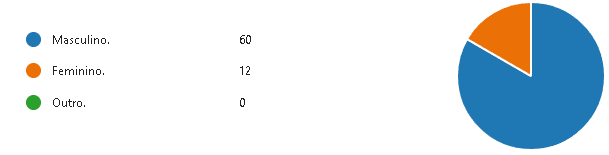
\includegraphics[scale=0.6]{figuras/1.png}
\caption{Questão 1}
\end{figure}

2. Qual disciplina você está cursando?

Nesta questão, sessenta e dois participantes responderam que estão cursando a disciplina de Requisitos de Software, enquanto apenas dez estão cursando a disciplina de Métodos de Desenvolvimento de Software.

\begin{figure}[H]
\centering
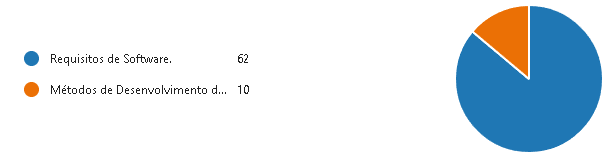
\includegraphics[scale=0.6]{figuras/2.png}
\caption{Questão 2}
\end{figure}

3. É sua primeira vez cursando a disciplina?

Dos setenta e dois participantes, sessenta e oito responderam que essa é a primeira vez que estão fazendo a mesma disciplina, enquanto apenas quatro estão refazendo a matéria.

\begin{figure}[H]
\centering
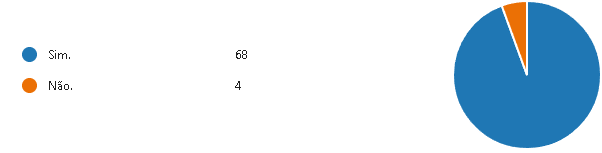
\includegraphics[scale=0.5]{figuras/3.png}
\caption{Questão 3}
\end{figure}

4. Você apresenta algum transtorno neurobiológico? (TDAH, TEA, distúrbios da aprendizagem, entre outros)

Nesta questão, nove participantes responderam que possuem algum tipo de transtorno neurobiológico, enquanto trinta e quatro responderam que não. Entretando, também possui uma parcela significativa de vinte e nove estudantes que não souberam responder sobre sua condição.

\begin{figure}[H]
\centering
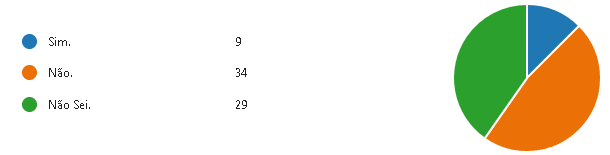
\includegraphics[scale=0.6]{figuras/4.png}
\caption{Questão 4}
\end{figure}

5. Menções (Exemplo: MM ou MS).

Referente ao retorno do feedback através apenas de menções, 56.9\% dos participantes votaram no valor 5, 29.4\% no valor 4, 11.1\% no valor 3, 1.4\% no valor 2 e 1.4\% no valor 1.

\begin{figure}[H]
\centering
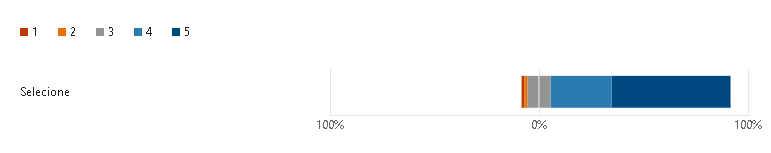
\includegraphics[scale=0.6]{figuras/5.png}
\caption{Questão 5}
\end{figure}

6. Visualizar o gabarito de cada questão.

Referente a visualização do gabarito de cada questão, 80.6\% dos participantes votaram no valor 5, 12.5\% no valor 4 e 6.9\% no valor 3, não existindo votos nos valores inferiores a 3, notando, assim, uma grande importância em saber qual é a resposta de determinada questão.

\begin{figure}[H]
\centering
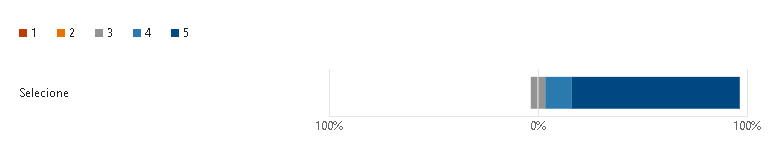
\includegraphics[scale=0.6]{figuras/6.png}
\caption{Questão 6}
\end{figure}

7. Exibir a explicação correspondente ao gabarito de cada questão.

Nesta questão, 75\% dos participantes votaram no valor 5, 16.7\% no valor 4, 6.9\% no valor 3 e 1.4\% no valor 2, não tendo respostas para o valor 1. Nota-se, então, um grande interesse na exibição de uma explicação para cada questão do questionário.

\begin{figure}[H]
\centering
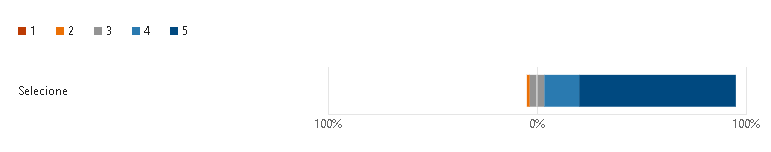
\includegraphics[scale=0.6]{figuras/7.png}
\caption{Questão 7}
\end{figure}


8. Indicação do material de estudo necessário para revisões do conteúdo.

Referente a indicação de material para estudo, 66.7\% dos participantes votaram no valor 5, 15.3\% no valor 4, 9.7\% no valor 3, 5.6\% no valor 2 e 2.8\% no valor 1. Com esses dados, é perceptivel o interesse por parte dos participantes na indicação de materias de estudo como complemento.

\begin{figure}[H]
\centering
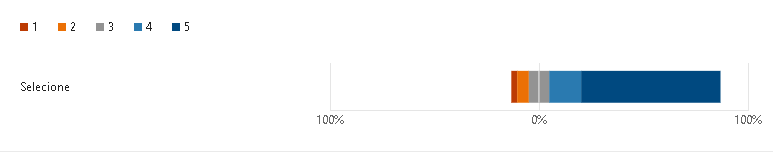
\includegraphics[scale=0.6]{figuras/8.png}
\caption{Questão 8}
\end{figure}

9. Visualizar os temas dos conteúdos que tiveram baixa taxa de acerto por meio de indicações textuais.

Referente a esta questão, 50\% dos participantes votaram no valor 5, 26.4\% no valor 4, 15.3\% no valor 3, 6.9\% no valor 2 e 1.4\% no valor 1.

\begin{figure}[H]
\centering
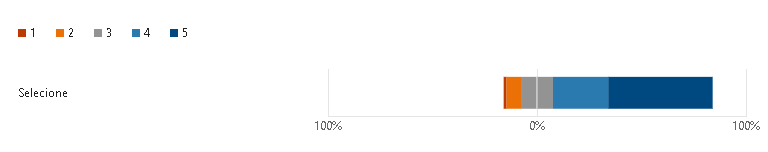
\includegraphics[scale=0.6]{figuras/9.png}
\caption{Questão 9}
\end{figure}

10. Visualizar um gráfico com uma divisão por temas em um conteúdo informando o desempenho na avaliação.

Quanto a este formato de feedback, 34.7\% dos participantes votaram no valor 5, 26.4\% no valor 4, 25\% no valor 3, 11.1\% no valor 2 e 2.8\% no valor 1. Nota-se que, comparado com as questões anteriores, não existe um grande interesse neste formato de feedback, podendo servir como feedback secundário.

\begin{figure}[H]
\centering
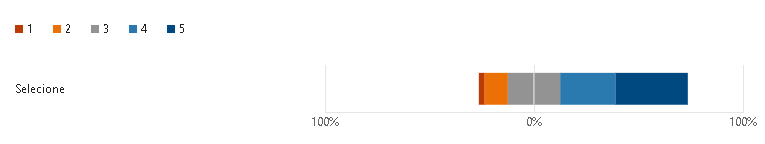
\includegraphics[scale=0.6]{figuras/10.png}
\caption{Questão 10}
\end{figure}

11. Reunião com o professor da disciplina para discutir sobre o resultado na avaliação e receber um Feedback humano.

Nesta questão, 22.2\% dos participantes votaram no valor 5, 19.4\% no valor 4, 43.1\% no valor 3, 8.3\% no valor 2 e 6.9\% no valor 1. Percebe-se um maior desinteresse por parte dos participantes neste formato de feedback, visto que mais de 50\% dos participantes votaram em um valor menor ou igual a três.

\begin{figure}[H]
\centering
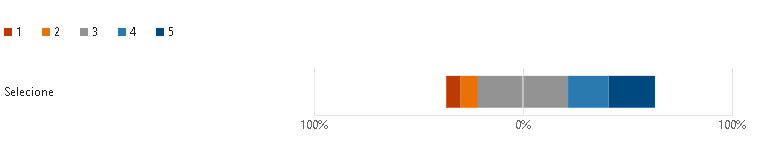
\includegraphics[scale=0.6]{figuras/11.png}
\caption{Questão 11}
\end{figure}

12. Relatório no formato PDF com um feedback descritivo do desempenho do aluno na avaliação. 

Para esta questão, 30.6\% dos participantes votaram no valor 5, 20.8\% no valor 4, 31.9\% no valor 3, 9.7\% no valor 2 e 6.9\% no valor 1. 

\begin{figure}[H]
\centering
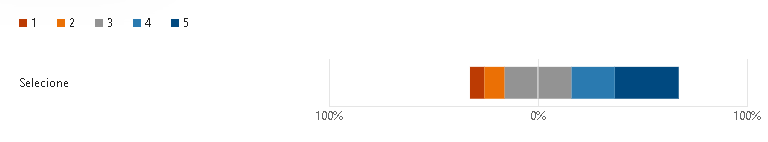
\includegraphics[scale=0.6]{figuras/12.png}
\caption{Questão 12}
\end{figure}
